\chapter{An Axiomatic Approach to Geometry}

The contents of this chapter are adapted Ardin's textbook \textit{Geometric Algebra} \cite{artin}.

\section{First Axiom}

\begin{definition}
    A plane is a triple $(\pt,\li,\icset).$ The set $\pt$ consists of the points, the set $\li$ consists of the lines, and the inclusion $\icset \subseteq \pt \times \li$ is an incidence relation. 
\end{definition}

\begin{definition}
    If $l,m \in \li$ such that either $l = m$ or $P \ic l \implies (P,m) \notin \icset \ \forall\, P \in \pt$, then we say $l$ and $m$ are parallel.
\end{definition}

\begin{axiom}[1]
    For any $P,Q \in \pt,$ there exists a unique $l \in \li$ such that $P \ic l$ and $Q \ic l.$ We write $l=P+Q.$
\end{axiom}

For any given $l,m \in \li$, if $\exists!\,P \in \pt$ such that $P \ic l$ and $P \ic m$, then $l \nparallel m$. If there are two or more such points, say $P$ and $Q$, then $P \ic l,$ $Q \ic l,$ $P \ic m,$ and $Q \ic m,$. By axiom 1, $l=m$ and hence, $l \parallel m$.

\vspace{1ex}

\noindent
Let $\pt_l \subset \pt$ be the set of all points on $l$ that is $\pt_l := \{ P \in \pt \colon P \ic l\}$.

\section{Second Axiom}

\begin{axiom}[2]
    For any $P \in \pt$ and $l \in \li,$ there exists a unique $m \in \li$ such that $P \ic m,$ and $l \parallel m.$
\end{axiom}

\begin{theorem}
    Parallel is an equivalence relation.
\end{theorem}
\begin{proof}
    For any $l \in \li$, $l=l$, hence $l \parallel l.$ If $l,m \in \li$ and $l \parallel m,$ then $m \parallel l.$ Assume $l \parallel m,$ and $m \parallel n$. If there exists no $P \in \pt$ such that $P \ic l$ and $P \ic n$, then $l \parallel n$. Otherwise, if $\exists\, P \in \pt$ such that $P \ic l$ and $P \ic n$, then by axiom 2, $\exists!\, r \in \li$ such that $P \ic r,$ and $ r \parallel m.$ Hence, $l=n$ and $l \parallel n.$
\end{proof}

\noindent
An equivalence class of parallel lines is called a pencil of parallel lines.

\begin{theorem} \label{thm:lines_num_pts}
    Suppose there exist three distinct pencils $\pi_1, \pi_2$ and $\pi_3$ of parallel lines. Then any pencil $\pi$ contains as many lines as the number of points on any line.
\end{theorem}
\begin{proof}
    Let $l \in \pi_1$, $m \in \pi_2.$ For every $Q_i \in \pt$ such that $Q_i \ic l$, by axiom 2, there exists exactly one $m_i \in \li$ such that $m \nparallel m_i.$ If $m_i = m_j$, by axiom 1, $P_i=P_j$ and therefore $i=j$.
    \vspace{1ex}

    \noindent
    For every $l_i \in \pi_2$, as $l \parallel l_i,$ there exists exactly one $P_i \in \pt$ such that $P_i \ic l$ and $P_i \ic l_i$. If $P_i = P_j$ and since $l_i \parallel l_j,$ by definition, $l_i=l_j$ and therefore $i=j.$ 

    We found a one-to-one correspondence between the points on $l$ and the lines in $\pi_2.$ Hence, for given two distinct pencils, the number of lines in one pencil is equal to the number of points on a line in another pencil. Now, we use the fact that we have 3 distinct pencils of parallel lines. The number of points on a line in $\pi_3$ is equal to the number of lines in $\pi_1$ and the number of points on a line in $\pi_3$ is equal to the number of lines in $\pi_2,$ hence the number of lines in $\pi_1$ and $\pi_2$ is equal and therefore, the number of points on any line in $\pi_1$, $\pi_2$ and $\pi_3$ is same.
\end{proof}

\section{Third Axiom}
\begin{axiom}[3]
    There exist three distinct points $A,B,C \in \pt$ such that $(C,A+B) \notin \icset$. We also say that there exist three non-collinear points.
\end{axiom}

\noindent
The smallest structure possible with this geometry is $\Z_2^2.$

\section{Fourth Axiom}
\begin{definition}
    A map $\sigma\colon \pt \to \pt$ is called a dilatation if for any distinct $P,Q \in \pt$ and $l' \in \li$ such that $l' \parallel P+Q$ and $P' \ic l'$, we have $Q' \ic l'$ where $P'=\sigma P$ and $Q'=\sigma Q$.
\end{definition}

\noindent
We can give two examples,
\begin{enumerate}[label=\roman*.]
    \item $\sigma P=P_0\ \forall\, P \in \pt$ and a fixed $P_0 \in \pt$.
    \item $\sigma P=P\ \forall\, P \in \pt$.
\end{enumerate}

\begin{theorem}
    A dilatation $\sigma$ is uniquely determined by the images $P', Q'$ of two distinct points $P$ and $Q$. If $P'=Q'$, then $\sigma$ is degenerate and all points are mapped to $P'$. Otherwise, if $P' \neq Q'$, then $\sigma$ is one-to-one and onto map.
\end{theorem}
\begin{proof}
    For $R \notin \pt_{P+Q}$, $R+P \nparallel R+Q$. Let $l' \in \li$ such that $P' \ic l'$ and $l' \parallel R+P$, then by definition, $R' \ic l'$. Similarily, let $l'' \in \li$ such that $Q' \ic l''$ and $l'' \parallel Q+P$, and so, $R' \ic l''$. Hence, $l' \nparallel l''$ and $\exists!\, R' \in \pt$ such that $R' \ic l'$ and $R' \ic l''$. Therefore, $R'$ is uniquely determined.

    \vspace{1ex}

    \noindent
    For $R \in \pt_{P+Q}$, $P \neq R$. By axiom 3, $\exists\, S \notin \pt_{P+Q}$. If $R \in \pt_{P+S}$, then $P+Q=P+S$ since $P,R \in \pt_{P+Q}$ and $P,R \in \pt_{P+S}$. Therefore, $R \notin \pt_{P+S}$. We uniquely determine $S'$ using the images $Q'$ and $P',$ and later uniquely determine $R'$ using the images $S'$ and $P'.$

    \vspace{1ex}

    Suppose $P' = Q'$. Then the degenerate map $\gamma$ which maps every point to $P'$ has the same effect as $\sigma$ which sends both $P$ and $Q$ to $P'$. Hence, $\sigma = \gamma$ due to uniqueness.

    \vspace{1ex}

    \noindent
    Suppose $P' \neq Q'$, and let $R'$ be a given point. For $R' \notin \pt_{P'+Q'}$, $R'+P' \nparallel R'+Q'$. Let $l_1 \in \li$ such that $P \ic l_1$ and $l_1 \parallel R'+P'$ and let $l_2 \in \li$ such that $Q \ic l_2$ and $l_2 \parallel Q'+P'$. Then, $l_1 \nparallel l_2$ and hence, $\exists!\,R \in \pt$ such that $R \ic l_1$ and $R \ic l_2$. Therefore, $R$ is uniquely determined.

    \vspace{1ex}

    If $R \in \pt_{P+Q}$, then $P \ic l_1$ and $Q \ic l_2$, hence $P+Q = l_1$ or $P+Q = l_2$. By definition, $P'+Q' \parallel P' + R'$ or $P'+Q' \parallel Q' + R'$, which contradicts. Hence, with the help of given images of $P$ and $Q$ and using the point, we found $R$. We conclude that $R'$ is the image of $R$. For $R' \in \pt_{P'+Q'}$, $P \neq R$. According to axiom 3, $\exists\, S' \notin \pt_{P'+Q'}$. If $R' \in \pt_{P'+S'}$,  then $P'+Q'=P'+S'$ since $P',R' \in \pt_{P'+Q'}$ and $P',R' \in \pt_{P'+S'}$. Therefore, suppose $R' \notin \pt_{P'+S''}$ and we uniquely determine $S$ whose image is $S'$ and prove that we can uniquely find $R$ whose image is $R'$ using the images $P'$ and $Q'$.
\end{proof}

\begin{definition}
    Let $\sigma$ be a non-degenerate dilatation and $P \in \pt$. Any $l \in \li$ such that $P \ic l$ and $\sigma P \ic l$ is called a trace of $P$. If $P = \sigma P$, then all the lines passing through $P$ are traces of $P$. Otherwise, if $P \neq \sigma P$, then the trace of $P$ is unique and is given by $P + \sigma P$. We denote the set of all traces of $\sigma$ for all $P \in \pt$ as $\zeta_\sigma$.
\end{definition}

\begin{theorem} \label{thm:dil_on_same_line}
    Let $\sigma$ be a non-degenerate dilatation, $P \in \pt$ and $l$ be a trace of $P$. If $Q \ic l$, then $\sigma Q \ic l$. 
\end{theorem}

\begin{proof}
    Assume $Q \neq P$ and take $l=P+Q$. Then $\sigma Q \neq \sigma P$ and by definition, $\sigma P + \sigma Q \parallel l$. But $\sigma P \ic \sigma P + \sigma Q$ and $ \sigma P \ic l$, hence, $l=\sigma P + \sigma Q.$ Therefore, $\sigma Q \ic l$.
\end{proof}

\begin{coro}
    The intersection of non-parallel traces is a fixed point.
\end{coro}

\noindent
This leaves us with three possibilities for the traces of non-singular dilatation, which are:
\begin{itemize}
    \item $\sigma=1,$ if and only if $\zeta_\sigma = \li$
    \item $\sigma \neq 1$ and if $P_0$ is a fixed point of $\sigma$, then $\zeta_\sigma = \{l=P_0+P\colon P \in \pt\}$
    \item $\sigma \neq 1$ and $\sigma$ fixes no point, then $\zeta_\sigma = \pi$, where $\pi$ is some pencil of parallel lines
\end{itemize}

\begin{definition}
    A non-singular dilatation $\tau$ is called a translation if either $\tau = 1$ or $\tau$ has no fixed point. If $\tau \neq 1,$ then traces of $\tau$ form a pencil $\pi$ of parallel lines which is called the direction of $\tau.$
\end{definition}

\begin{theorem}
    A translation $\tau$ is uniquely determined by the image $P'$ of one point $P.$
\end{theorem}

\begin{proof}
    Let $l \in \zeta_\tau$ such that $P \ic l.$ For some $Q \notin \pt_l$, let $l' \parallel l$ and $Q \ic l'$, then $l' \in \zeta_\tau$ and $\tau Q \ic l$ since $\zeta_\tau$ is a penci since $\zeta_\tau$ is a pencill.  Let $m,m' \in \li$ such that $m=P+Q$, $P' \ic m'$ and $m' \parallel m$. Then by definition, $ \tau Q \ic m'$. Since $l \not \parallel m$, we have $l' \not \parallel m'$. Since $\tau Q \ic m'$ and $\tau Q \ic l'$, therefore $\tau Q$ is uniquely determined.

    \vspace{1ex}

    For $Q \in \pt_l$ and $Q \neq P$, $\exists\, S \notin \pt_{l}$ by axiom 3. Let $l'' \parallel l$ such that $S \ic l''$ and hence, $l'' \in \zeta_\tau$ and $\tau S \ic l''$.  Let $n,n' \in \li$ such that $n=P+S$, $P' \ic n'$ and $n' \parallel n$. Then by definition, $ \tau S \ic m'$. Since $l \not \parallel n$, we have $l' \not \parallel n'$. Since $\tau S \ic m'$ and $\tau S \ic l'$, therefore $\tau S$ is uniquely determined and using $\tau S$, we can uniquely determine $\tau Q$.
\end{proof}

\begin{theorem}
    Dilatations form a group $D$ and translations form a normal subgroup $T$ of $D$. If $\sigma$ is a dilatation and $\tau \neq 1$ is a translation, then $\tau$ and $\sigma \tau \sigma^{-1}$ have the same direction.
\end{theorem}
\begin{proof}
    Let $\sigma_1, \sigma_2$ be two dilatations. Then, their composition is also
    a dilatation since
    \[ P+Q \parallel \sigma_2 P + \sigma_2 Q \parallel \sigma_1 \sigma_2 P+ \sigma_1 \sigma_2 Q \]
    The identity map is a dilatation and since dilatations are one-one and onto, $\sigma^{-1}$ exists and is a dilatation because
    \[ \sigma^{-1}P+\sigma^{-1}Q \parallel \sigma\sigma^{-1}P+\sigma\sigma^{-1}Q = P+Q \]
    Associativity directly follows from function composition. Hence, dilatations form a group under function composition.

    Let $\tau$ be a translation. Suppose $\tau^{-1}$ fixes a point $P$ i.e. $\tau^{-1}P=P \implies P=\tau P$. Therefore, $\tau = 1$ and $\tau_{-1}=1$ i.e. $\tau^{-1}$ fixes no point iff $\tau^{-1} \neq 1$. This proves that $\tau^{-1}$ is a translation.

    \vspace{1ex}

    \noindent
    Given two translations $\tau_1$ and $\tau_2$, suppose $\tau_1 \tau_2$ fixes a point. Then,
    \[ \tau_1 \tau_2 P=P \implies \tau_2 P= \tau_1^{-1}P \]
    So, $\tau_1^{-1} =\tau_2$ and hence, $\tau_1 \tau_2=1$. Thus $\tau_1 \tau_2$ fixes no points iff $\tau_1 \tau_2 \neq 1$ .
    Therefore, translations form a subgroup of dilatations.

    \vspace{1ex}

    \noindent
    Let $\sigma$ be a dilatation and $\tau$ be a translation. Suppose $\sigma \tau \sigma^{-1}$ fixes a point $P$. Then,
    \[ \sigma \tau \sigma^{-1}P=P \: \Rightarrow \tau \sigma^{-1}P=\sigma^{-1}P \]
    i.e. $\tau$ fixes a point $\sigma^{-1}P$ and hence $\tau_1$. Thus, $\sigma \tau \sigma^{-1}$ fixes no points iff $\sigma \tau \sigma^{-1} \neq 1$ i.e. $\tau = 1$. So, $\sigma \tau \sigma^{-1}$ is a translation and hence the subgroup of translations is normal.

    \vspace{1ex}

    \noindent
    Suppose $\tau \neq 1$ and the pencil $\pi$ is the direction of $\tau$. Then, $\tau \sigma^{-1}P+\sigma^{-1}P$ is the $\tau$-trace of $\sigma^{-1}P$ and
    \[ \tau \sigma^{-1}P+\sigma^{-1}P \parallel \sigma \tau \sigma^{-1}P+ \sigma \sigma^{-1}P = \sigma \tau \sigma^{-1}P+ P \]
    This shows $\sigma \tau \sigma^{-1}$ and $\tau$ have the same direction.
    
\end{proof}

\begin{theorem}
    Identity dilatation along with the translations with same pencil $\pi$ as their direction form a group.
\end{theorem}

\begin{proof}
    For  $\tau \neq 1$, $P + \tau P \parallel \tau P + \tau^{-1} \tau P$. Hence, $\tau$ and $\tau^{-1}$ have the same direction. For $\tau_1, \tau_2 \neq 1$ such that they have the same direction $\pi$. By Theorem \ref{thm:dil_on_same_line}, $P$, $\tau_2 P$ and $\tau_1 \tau_2 P$ lie on the same line. If $\tau_1 \tau_2 P = P$, then $\tau_1 \tau_2 = 1$  and if $\tau_1 \tau_2 P \neq P$, then $\tau_1 \tau_2$ have the same direction $\pi.$
\end{proof}

\begin{theorem}
    If translations with different directions exist, then $T$ is a commutative group.
\end{theorem}

\begin{proof}
    Suppose $\tau_1$ and $\tau_2$ have different directions. Then, the translations $\tau_1 \tau_2 \tau_1^{-1}$, $\tau_2$ and $\tau_2^{-1}$ have the same direction. If $\tau_1 \tau_2 \tau_1^{-1}\tau_2^{-1} \neq 1$, then $\tau_1 \tau_2 \tau_1^{-1}\tau_2^{-1}$ has the same direction as $\tau_2$. Further, $\tau_1$, $\tau_1^{-1}$ and $\tau_2 \tau_1^{-1}\tau_2^{-1}$ have the same direction, hence $\tau_1 \tau_2 \tau_1^{-1}\tau_2^{-1}$ has the same direction as $\tau_1$. But $\tau_1$ and $\tau_2$ have different directions, hence $\tau_1 \tau_2 \tau_1^{-1}\tau_2^{-1} =1$ i.e.  $\tau_1 \tau_2=\tau_2 \tau_1$.

    \vspace{1ex}

    Suppose $\tau_1$ and $\tau_2$ have the same direction. By assumption, there exists $\tau_3$ which has a direction different $\tau_1 $ and $\tau_2$. Hence, $\tau_1 \tau_3 = \tau_3 \tau_1$ from above. Now, $\tau_2 \tau_3$ will have a direction different from $\tau_1$ otherwise $\tau_2^{-1} \tau_2 \tau_3 = \tau_3$ will have the same direction as $\tau_1$. Thus
    \[ (\tau_1 \tau_2 ) \tau_3 = \tau_1 (\tau_2\tau_3) = (\tau_2 \tau_3) \tau_1 = \tau_2 (\tau_3 \tau_1) = \tau_2 (\tau_1 \tau_3) = (\tau_2 \tau_1) \tau_3 \]
    Hence, $\tau_1 \tau_2=\tau_2 \tau_1$.
\end{proof}

\begin{axiom}[4a]
    For any $P,Q \in \pt$, there exists a translation $\tau_{PQ}$ which moves P to Q i.e. $\tau_{PQ}(P)=Q.$ 
\end{axiom}

\begin{definition}
    A map $\alpha : T \to T$ is called a trace preserving homomorphism if:
    \begin{enumerate}[label=\roman*.]
        \item it is a homomorphism of T i.e. $(\tau_1\tau_2)^{\alpha} = \tau_1^{\alpha}\tau_2^{\alpha} $
        \item it preserves traces i.e. either $\tau^{\alpha} = 1$ or $\tau$ and $\tau^{\alpha}$ have the same direction.
    \end{enumerate}
\end{definition}

\noindent
We call the set of trace preserving homomorphisms $k$.

\begin{definition}
    Given $\alpha, \beta \in k$, we define $\alpha + \beta$ and $\alpha \cdot \beta$ such that
    \[ \tau^{\alpha+\beta} = \tau^{\alpha} \tau^{\beta} \]
    \[ \tau^{\alpha \cdot \beta} = (\tau^{\alpha} )^{\beta} = \tau^{\alpha \beta} \]
\end{definition}

\noindent
We define $0 \in k$ as the map that sends all translations to the identity dilatation.

\begin{theorem}
    $\langle k, +, \cdot\rangle$ is a ring with identity. \cite[Thm.~2.9]{artin}
\end{theorem}

\begin{theorem}
    Let $\alpha \in k$, $\alpha \neq 0$ and let $P \in \pt$. There exists a unique dilation $\sigma$ which fixes $P$ and
    \[ \tau^\alpha = \sigma \tau \sigma^{-1}\ \forall\,\tau\in T \]
\end{theorem}

\begin{proof}
    Suppose such a $\sigma$ exists. For any $Q \in \pt$, and hence by axiom 4(a), we know there exists a $\tau_{PQ} \in T$ such that $\tau_{PQ}(P)=(Q)$. Then $\tau_{PQ}^\alpha = \sigma \tau_{PQ} \sigma^{-1}$.
    \[ 
    \tau_{PQ}^\alpha(P) = \sigma \tau_{PQ} \sigma^{-1}(P) = \sigma \tau_{PQ}(P) = \sigma (Q)
    \]
    Since we know the images of two points, hence it uniquely determines $\sigma$.

    \noindent
    Let $\alpha \in k$ and $Q, R \in \pt$ such that $Q \neq R$. Then, 
    \[ \tau_{QR}\tau_{PQ}=\tau_{PR} \implies \tau_{QR}^\alpha\tau_{PQ}^\alpha=\tau_{PR}^\alpha \]
    and
    \[ \tau_{QR}^\alpha(\tau_{PQ}^\alpha (P))=\tau_{PR}^\alpha(P) \implies \tau_{QR}^\alpha(\sigma(Q))=\sigma(R) \]   
    Now, we need to prove that $\sigma$ is a dilatation. Let $l \in \li$ such that $\sigma(Q) \ic l$ and $l \parallel Q+R$. Hence, $l \in \zeta_{\tau_{QR}}$ and $l \in \zeta_{\tau_{QR}^{\alpha}}$. By Theorem \ref{thm:dil_on_same_line}, we have $\sigma(R) \ic l$. So, $Q+R \parallel \sigma(Q)+ \sigma(R)$.
    Since we know the images of two points under $\sigma$, hence $\sigma$ is uniquely determined.

    \vspace{1ex}

    Since $\sigma(P) = \tau_{PP}^\alpha(P)=P$, $\sigma$ fixes P. If $\sigma$ is degenerate, then every point is mapped to P i.e. $\sigma(Q) = \tau_{PQ}^{\alpha}(P) = P \implies \tau_{PQ}^{\alpha} = 1\ \forall\, Q \in \pt$. Therefore, $\tau^\alpha = 1$, for all $\tau \in T$ and hence $\alpha=0$. Thus $\sigma$ can't be degenerate and
    \[
    \sigma(Q)=\tau_{PQ}^{\alpha}(P)= \tau_{PQ}^{\alpha}(\sigma(P)) \: \Rightarrow Q = \sigma^{-1}\tau_{PQ}^{\alpha}\sigma(P)
    \]
    So, $\sigma^{-1}\tau_{PQ}^{\alpha}\sigma$ is a translation which maps $P$ to $Q$ and it is uniquely determined as $\tau_{PQ}$ since translations are uniquely determined by image of one point. Thus
    \[
    \sigma^{-1}\tau_{PQ}^{\alpha}\sigma = \tau_{PQ} \: \Rightarrow \tau_{PQ}^{\alpha} = \sigma\tau_{PQ}\sigma^{-1}
    \]
    Since the point Q was chosen arbitrarily, $\tau_{PQ}$ can be any translation. Therefore,
    \[
    \tau^{\alpha} = \sigma\tau\sigma^{-1} \: \: \forall \; \tau \in T
    \]
\end{proof}

\begin{axiom}[4b]
    If $\tau_1, \tau_2 \in T$ such that $\zeta_{\tau_1} = \zeta_{\tau_2}$ and $\tau_1 \neq 1$, there exists $\alpha \in k$ such that $\tau_2 = \tau_1^\alpha$.
\end{axiom}

\begin{axiom}[4b $P$]
    (For a given $P \in \pt$) For any $Q,R \in \pt$ such that $P$, $Q$ and $R$ are distinct and collinear, there exists a dilatation $\sigma$ which fixes $P$ and maps $Q$ to $R$.
\end{axiom}

\begin{theorem}
    If axiom 4b $P$ holds for some $P \in \pt$, then axiom 4b is true, and axiom 4b implies 4b $P$ for all $P \in \pt.$
\end{theorem}

\begin{proof}
    Assume axiom 4b P is true for a given $P \in \pt.$ Let $\tau_1, \tau_2 \in T$ such that $\zeta_{\tau_1} = \zeta_{\tau_2}$, $\tau_1(P)=Q$, and $\tau_2(P)=R$. Let $\sigma$ be the dilatation for which $\sigma(P)=P$ and $\sigma(Q)=R$. Now, $\sigma\tau_1\sigma^{-1} \in T$ and $\sigma\tau_1\sigma^{-1}(P) = \sigma\tau_1(P)=\sigma(Q)=R. $ Hence, $\sigma\tau_1\sigma^{-1} = \tau_{PR}=\tau_2$. So, we have $\alpha \in k$ such that $\tau^\alpha = \sigma\tau\sigma^{-1}$ and therefore $\tau_2=\tau_1^\alpha.$

    Assume axiom 4b is true and let $P,Q,R \in \pt$ be distinct and collinear. Consider $\tau_1=\tau_{PQ}$, $\tau_2=\tau_{PR}$ such that $\zeta_{\tau_1} = \zeta_{\tau_2}$. By axiom 4b, there exists a $\alpha \in k$ such that $\tau_2=\tau_1^\alpha$. From the previous theorem, there exists a dilatation $\sigma$ for $\alpha$ such that $\sigma(P)=P$ and $\tau^{\alpha} = \sigma\tau\sigma^{-1}$ for all $\tau \in T.$ Therefore,
    \[
    \tau_2=\sigma\tau\sigma^{-1} \: \Rightarrow \tau_2\sigma=\sigma\tau_1
    \]
    Hence, $\sigma$ is the desired dilatation. So, axiom 4b $P$ holds for all $P \in \pt$.
\end{proof}

\section{Desargues' Theorem}

Assuming only the first three axioms hold. 

\begin{theorem}[Desargues' Theorem]
    Let $l_1, l_2, l_3$ be distinct lines which are either parallel or meet at a point $P$. Let $Q, Q'$ be points on $l_1$; $R, R'$ points on $l_2$ and $S, S'$ points on $l_3$ which are distinct from $P$ if the lines meet.
    \[
    \text{If } \: \: Q+R \parallel Q'+R' \: \:  \text{ and } \: \: Q+S \parallel Q' +S'\text{,}
    \]
    \[
    \text{then} \: \: R+S \parallel R'+S'
    \]
\end{theorem}

\begin{figure}[H]
    \begin{center}
        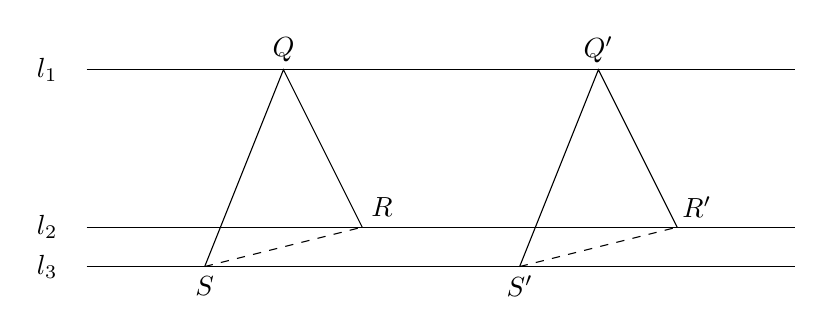
\begin{tikzpicture}
            \draw (0.5,0.5) -- (9.5,0.5);
            \draw (0.5,1) -- (9.5,1);
            \draw (0.5,3) -- (9.5,3);
            \draw[dashed] (2,0.5) -- (4,1);
            \draw[dashed] (6,0.5) -- (8,1);
            \draw (2,0.5) -- (3,3) -- (4,1);
            \draw (6,0.5) -- (7,3) -- (8,1);
            \draw (0,3) node {$l_1$};
            \draw (0,1) node {$l_2$};
            \draw (0,0.5) node {$l_3$};
            \draw (2,0.25) node {$S$};
            \draw (4.25,1.25) node {$R$};
            \draw (3,3.25) node {$Q$};
            \draw (6, 0.25) node {$S'$};
            \draw (8.25,1.25) node {$R'$};
            \draw (7,3.25) node {$Q'$};
        \end{tikzpicture}
    \end{center}
    \caption{Desargues' Theorem for case $\mathbf{D_a}$}
\end{figure}
\begin{figure}[H]
    \begin{center}
        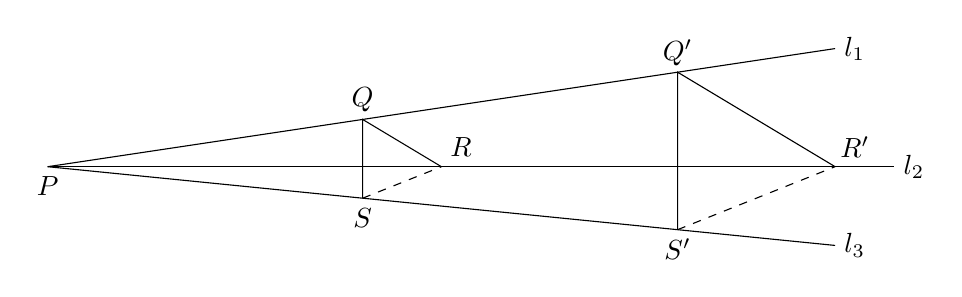
\begin{tikzpicture}
            \draw (0,0) -- (10.75,0);
            \draw (0,0) -- (10,-1);
            \draw (0,0) -- (10,1.5);
            \draw (4,-0.4) -- (4,0.6) -- (5,0);
            \draw (8,-0.8) -- (8,1.2) -- (10,0);
            \draw[dashed] (4,-0.4) -- (5,0);
            \draw[dashed] (8,-0.8) -- (10,0);
            \draw (11,0) node {$l_2$};
            \draw (10.25,-1) node {$l_3$};
            \draw (10.25,1.5) node {$l_1$};
            \draw (4,-0.65) node {$S$};
            \draw (5.25,0.25) node {$R$};
            \draw (4,0.85) node {$Q$};
            \draw (8,-1.05) node {$S'$};
            \draw (10.25,0.25) node {$R'$};
            \draw (8,1.45) node {$Q'$};
            \draw (0,-0.25) node {$P$};
        \end{tikzpicture}
    \end{center}
    \caption{Desargues' Theorem for case \textbf{DP}}
\end{figure}

\noindent
Let us discuss some trivial cases, 
\begin{itemize}
    \item If $Q'=Q,$ then $Q+R=Q'+R'$ and since $R \ic l_2, \ R' \ic l_2$ and $R \ic Q+R,$  hence $R=R'$ is uniquely determined. Hence, it follows that $S=S'.$
    \item If $Q, \ R, \ S \in \pt$ are collinear, hence the images $Q', \ R', \ S'$ are also collinear.
\end{itemize}
We will refer to the case when the lines $l_1, \ l_2, \ l_3$ are parallel as $\mathbf{D_a},$ and the case when the lines $l_1, \ l_2, \ l_3$ meet at point $P$ as $\mathbf{DP}.$

\begin{theorem}
    Axiom 4a implies $\mathbf{D_a}$ and axiom 4b P implies $\mathbf{DP}$.
\end{theorem}

\begin{proof}
    To prove $\mathbf{D_a}$, let $\tau$ be a translation which maps $Q$ to $Q'$. By definition, $Q'+R' \parallel Q+R \parallel \tau Q + \tau R = Q' + \tau R$. Therefore, $Q'+ R' = Q'+\tau R$. Since $l_2 \parallel Q+Q'$, we have $l_2 \in \zeta_\tau$ and $\tau R \ic l_2$. Therefore, $\tau R=R'$. Similarly, we get $\tau S = S'$. Thus, $R+S \parallel \tau R + \tau S \parallel R'+S'$.

    \vspace{1ex}

    To prove $\mathbf{DP}$, let $\sigma$ be a dilatation which fixes $P$ and maps $Q$ to $Q'$. By definition, $Q'+R' \parallel Q+R \parallel \sigma Q + \sigma R = Q' + \sigma R$. Therefore $Q'+ R' = Q'+\sigma R$. Since $l_2 = P+R$, we have $l_2 \in \zeta_\sigma$ and $\sigma R \ic l_2$. Therefore, $\sigma R=R'$. Similarly, we get $\sigma S = S'$. Thus, $R+S \parallel \sigma R + \sigma S \parallel R'+S'$.
\end{proof}

\begin{theorem}
    $\mathbf{D_a}$ implies axiom 4a and $\mathbf{DP}$ axiom 4b P. 
\end{theorem}

\begin{proof}
    Suppose each line contains only two points. Then by Theorem \ref{thm:lines_num_pts}, there are two lines in a given pencil of parallel lines. Hence, only four points exists in a given pencil in our geometry. This resembles the smallest geometry that we know in which first three axioms hold, $\Z_2^2$. Let the four points of the geometry be $A$, $B$, $C$ and $D$. Then there are six lines, namely $A+B$, $A+C$, $A+D$, $B+C$, $B+D$ and $C+D$. This geometry satisfies all axioms, inluding axioms 4a and 4b. Thus from now on, we'll assume that each line contains at least three points and that for any given two lines, there exists a point such that it doesn't lie on either of the lines.
 
    Assuming $\mathbf{D_a}$, let any $Q, \ Q' \in \pt$ such that $Q \neq Q'$. Consider a map $\eta_Q$ which maps $Q$ to $Q'$ and is only defined for any $R \in \pt$ such that $(R,Q+Q') \notin \icset$. Let $l \in \li$ such that $\ l \parallel Q+Q'$ and $R\ic l$. Then $l \neq Q+Q'$. Similarily, let $m \in \li$ such that $m \parallel Q+R$ and $Q' \ic m$ which gives $m \neq Q+R$. Since $Q+Q' \not \parallel Q+R,$ we have $l \not \parallel m$. Let $R' \in \pt$ such that $R' \ic l$ and $R' \ic m$. Hence, $R' \neq Q'$ and $R' \neq R$. In simpler terms, $R+R' \parallel Q+Q'$ and $Q+R \parallel Q' + R'$, these describe the image $R'$ of $R$ under the map $\eta_Q.$

    \begin{figure}[H]
        \begin{center}
         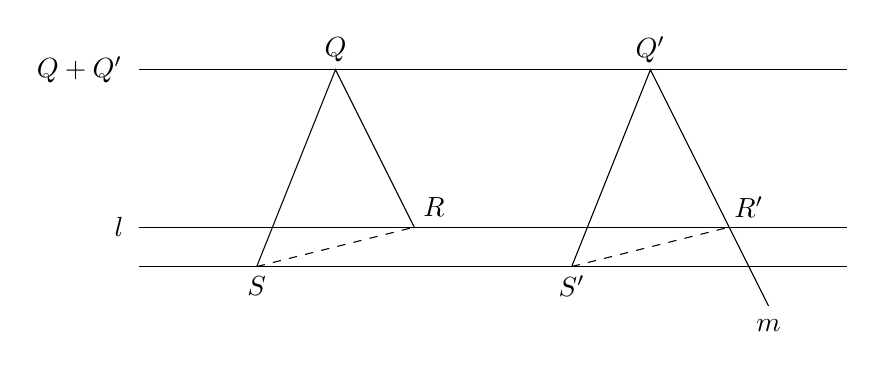
\begin{tikzpicture}
          \draw (0.5,0.5) -- (9.5,0.5);
          \draw (0.5,1) -- (9.5,1);
          \draw (0.5,3) -- (9.5,3);
          \draw[dashed] (2,0.5) -- (4,1);
          \draw[dashed] (6,0.5) -- (8,1);
          \draw (2,0.5) -- (3,3) -- (4,1);
          \draw (6,0.5) -- (7,3) -- (8.5,0);
          \draw (-0.25,3) node {$Q+Q'$};
          \draw (0.25,1) node {$l$};
          \draw (8.5,-0.25) node {$m$};
          \draw (2,0.25) node {$S$};
          \draw (4.25,1.25) node {$R$};
          \draw (3,3.25) node {$Q$};
          \draw (6, 0.25) node {$S'$};
          \draw (8.25,1.25) node {$R'$};
          \draw (7,3.25) node {$Q'$};
         \end{tikzpicture}
        \end{center}
        \caption{}
    \end{figure}

    Since we have $R$ and $R'$, we can now construct a map $\eta_R$ which maps $R$ to $R'$. With similar construction, it will send $Q$ to $Q'$. Similarily, we'll find the image of any $S \in \pt$ such that $(S, R+R') \notin \icset$, and $(S, Q+Q') \notin \icset$. Thus $S+S' \parallel Q+Q' \parallel R+R'$, $Q+R \parallel Q'+R'$ and $Q+S \parallel Q'+S'$. So, we can uniquely determine the image $S'$ under the map $\eta_Q$. By $\mathbf{D_a}$, $R+S \parallel  R'+S'$. Since $S+S' \parallel R+R'$ and $R+S \parallel  R'+S'$, $S'$ is also an image under the map $\eta_R$. Clearly, $\eta_Q$ and $\eta_R$ agree on any $S \in \pt$ such that $(S, R+R') \notin \icset$, and $(S, Q+Q') \notin \icset$.

    We now have $S$ and $S'$; we'll construct a map $\eta_S$, which maps $S$ to $S'.$ With similar construction, it will send $Q$ to $Q'$ and $R$ to $R'$. So, $\eta_Q$, $\eta_R$ and $\eta_S$ will agree on any $T \in \pt$ such that $(T, S+S') \notin \icset$, $(T, R+R') \notin \icset$ and $(T, Q+Q') \notin \icset$. The desired map $\tau$ is then a combination of the three maps -- for any point $T$, the image shall be the image under one of the three maps (for whichever it is defined). This map $\tau$ has the property that $\tau(Q) = Q$'.
    
    Now, we need to show that $\tau$ is a dilatation. Let any $U,V \in \pt$ such that one of the lines $Q+Q'$, $R+R'$ or $S+S'$ doesn't contain $U$ and $V$. Without loss of generality, let us assume that $Q+Q'$ is such a line, i.e. $(U,Q+Q') \notin \icset$ and $(V, Q+Q') \notin \icset$. Hence, we will use the map $\eta_Q$ to determine the image of $U$ and $V$. For $U+V \parallel Q+Q'$, we have $U' \ic U+V$, $V' \ic U+V$ and  $U'+V'=U+V$. For $U+V \not\parallel Q+Q'$, we'll use the same construction as we did to find the images of $R$ and $S$ and find images of $U$ and $V$ proving that $U+V \parallel U'+V'$. Hence, $\tau$ is a dilatation and therefore a translation as $\zeta_\tau$ is a pencil of parallel lines.

    Assuming $\mathbf{DP}$, let any distinct and collinear points $P,Q,Q' \in \pt$. We'll associate a map $\nu_Q$ which fixes P, maps $Q$ to $Q'$ and is only defined $\forall\, R \in \pt$ such that $(R,Q+Q') \notin \icset$. Take $l=P+R$, then $l \neq Q+Q'$. Let $m \in \li$ such that $m \parallel Q+R$, $Q' \ic m$ and $m \neq Q+R$. Since $P+R \not \parallel Q+R$, we have $l \not \parallel m$. Let $R' \in \pt$ such that $R' \ic l$ and $R' \ic m$. Thus $R' \neq Q'$ and $R' \neq R$. In simpler terms, $P \ic R+R'$ and $Q+R \parallel Q' + R'$, these describe the image $R'$ of $R$ under the map $\eta_Q.$

    \begin{center}
        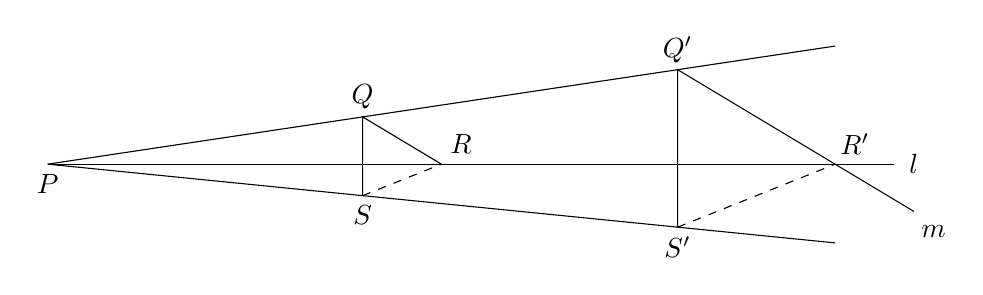
\begin{tikzpicture}
            \draw (0,0) -- (10.75,0);
            \draw (0,0) -- (10,-1);
            \draw (0,0) -- (10,1.5);
            \draw (4,-0.4) -- (4,0.6) -- (5,0);
            \draw (8,-0.8) -- (8,1.2) -- (11,-0.6);
            \draw[dashed] (4,-0.4) -- (5,0);
            \draw[dashed] (8,-0.8) -- (10,0);
            \draw (11,0) node {$l$};
            \draw (11.25,-0.85) node {$m$};
            \draw (4,-0.65) node {$S$};
            \draw (5.25,0.25) node {$R$};
            \draw (4,0.85) node {$Q$};
            \draw (8,-1.05) node {$S'$};
            \draw (10.25,0.25) node {$R'$};
            \draw (8,1.45) node {$Q'$};
            \draw (0,-0.25) node {$P$};
        \end{tikzpicture}
    \end{center}

    Since we have $R$ and $R'$, we can now construct a map $\nu_R$, which takes $R$ to $R'$. With the same construction, it will also send $Q$ to $Q'$. Similarily, we'll find the image of any $S \in \pt$ such that $(S, R+R') \notin \icset$ and $(S, Q+Q') \notin \icset$. Thus $(P, Q+Q'), (P,R+R'), (P,S+S') \in \ic$, $Q+R \parallel Q'+R'$ and $Q+S \parallel Q'+S'$. So, we can uniquely determine the image $S'$ under the map $\nu_Q$. By $\mathbf{DP}$, we have $R+S \parallel  R'+S'$. Since $P\ic S+S'$ and $R+S \parallel R'+S'$, $S'$ is also an image under the map $\nu_R$. Clearly, $\nu_Q$ and $\nu_R$ agree on $S \in \pt$ such that $(S, R+R') \notin \icset$ and $(S, Q+Q') \notin \icset$.

    We now have $S$ and $S'$; we'll construct a map $\nu_S,$ which maps $S$ to $S'$. With similar construction, it will also send $Q$ to $Q'$ and $R$ to $R'$. So, $\nu_Q$, $\nu_R$ and $\nu_S$ agree on any $T \in \pt$ such that $(T, S+S') \notin \icset$, $(T, R+R') \notin \icset$ and $(T, Q+Q') \notin \icset$. The desired map $\sigma$ is then a combination of the three maps: for any point $T$ the image shall be the image under one of the three maps (for whichever it is defined) . This map $\sigma$ has the property that $\sigma(Q) = Q$'.
    
    Now, we need to show that $\sigma$ is a dilatation.  Let any $U,V \in \pt$ such that one of the lines $Q+Q'$, $R+R'$ or $S+S'$ doesn't contain $U$ and $V$. Without loss of generality, let us assume that $Q+Q'$ is such a line i.e. $(U,Q+Q') \notin \icset$ and $(V, Q+Q') \notin \icset$. Hence, we will use the map $\nu_Q$ to determine the image of $U$ and $V$. For $(P, U+V) \in \icset$, we have $U'\ic U+V$, $V' \ic U+V$ and $U'+V'=U+V$. For $(P, U+V) \notin \icset$, we'll use the same construction as we did to find the images of $R$ and $S$ and find images of $U$ and $V$ proving that $U+V \parallel U'+V'$. Hence $\sigma$ is the desired dilatation.
\end{proof}

In the light of the above two theorems, Desargues' theorem is a geometric equivalent of axioms 4a and 4b P.
